\section{Overview}
\label{sec:inference:overview}

Figure \ref{fig:overview_app} shows a high-level overview of the entire application consisting of these four parts:
\begin{enumerate}
  \item Camera Library (\texttt{libcamera.so})
  \item Python Package (\texttt{fhnwtoys})
  \item User Interface Class (\texttt{ui.py})
  \item Inference Application (\texttt{aionfpga.py})
\end{enumerate}

The camera interface is written in C++ and compiled into a shared library (\texttt{.so}).
This allows the inference application to load the camera library into its memory space (see section \ref{sec:inference:camera_library}).

The \texttt{fhnwtoys} Python package provides access to various settings and constants.

The \acrlong{ui} class serves as an interface between the inference application and the display.
It features two methods to easily update the user interface screens.

The inference application itself uses the other three components to acquire frames, run inference and display the classification results on the screen.

\begin{figure}
  \centering
  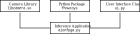
\includegraphics[width=\textwidth]{overview_app}
  \caption{High-level overview of the entire application}
  \label{fig:overview_app}
\end{figure}
